\chapter{Background}

\section{Memory structure}
Memory is one of the most critical components from a security point of view in a computer system, since during program execution it contains not only the data being processed but also the information necessary to determine the program's behavior. This includes:
\begin{itemize}
    \item \textbf{variables} containing temporary data used by the executed program(s);
    \item \textbf{data structures}, relationships between different types of objects for the purpose of managing more complex data;
    \item \textbf{pointers with memory addresses} which tell the program "where" a certain resource is. They can point:
    \begin{itemize}
        \item to other objects, to allow the program to read or write data;
        \item to functions, to allow the program to execute instructions located at a specific position;
    \end{itemize}
    \item \textbf{information used to manage the execution flow}, such as the address of the first instruction that needs to be executed when returning from a function call.
\end{itemize}
Unauthorized access to or arbitrary modification of these elements can therefore have consequences ranging from simple data corruption or program crashes to changes in the control flow and, in the most severe cases, the execution of unauthorized operations, which is the subject we're going to examine. To understand the origin and effects of the main memory corruption vulnerabilities, it is therefore useful to first consider how the memory space associated with a program is organized into its main regions. 

\clearpage
\begin{figure}[h]
    \centering
    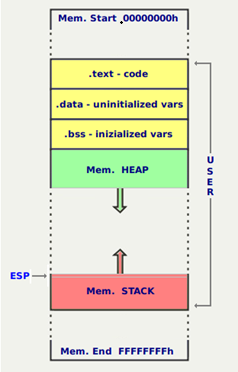
\includegraphics{images/stack-heap.png}
    \caption{Structure of memory areas.}
    \label{fig:stack_heap}
\end{figure}

\noindent The two areas primarily affected by attacks of this kind are the stack and the heap.

\subsection{Stack}
The stack is a data structure organised according to a LIFO (Last In, First Out) policy and used primarily for managing function calls. Each function call involves the creation of a \emph{stack frame} containing local variables, parameters and return information (such as the return address, which tells the program the point in the calling code from which to resume execution once the function has been exited). The allocation and deallocation of memory on the stack are automatic and handled by the compiler: when a function terminates, its corresponding frame is removed.

\subsection{Heap}
The heap is a memory region used for dynamic allocations, managed explicitly by the programmer using primitives such as \texttt{malloc}/\texttt{free} in C or \texttt{new}/\texttt{delete} in C++. These functions do not normally request a new memory region from the operating system for every individual location, but a user-space memory allocator manages larger regions of memory, dividing them into smaller blocks and keeping track of which portions are currently allocated or available for reuse.

On Linux systems, the allocator can obtain additional virtual memory from the kernel through mechanisms such as \texttt{brk()}, which changes the end of the process data segment, or \texttt{mmap()}, which creates new memory mappings. Large allocations are commonly serviced through \texttt{mmap()} while other allocations may be satisfied from memory already managed by the allocator or from an enlarged process heap. The exact strategy is implementation-dependent and may change according to allocation size and configuration. \cite{bib:gnu-allocator} \cite{bib:malloc-efficiency}

Unlike the stack, therefore, heap allocations do not follow a strict LIFO (Last In, First Out) order: allocated blocks may be released independently and subsequently reused for other object, which is essential for dynamically sized and long-lived data structures, but it also makes object lifetime and memory reuse more difficult to manage correctly, creating the conditions in which errors like UAF may appear.

\subsection{Pointers}\label{pointers}
In memory-unsafe languages, pointers are identifiers that may contain the address of a specific memory area (to which they "point") and, for example in C, are initialised using the \texttt{malloc} function and freed using the \texttt{free} function. The programmer can use them to perform operations both on the addresses they contain and on the values contained in the memory cells they point to.

Given their nature, they are one of the main vectors for memory-related attacks. We therefore introduce the concept of a \textbf{dangling pointer} \cite{bib:dangling-pointer}: a pointer, if manipulated incorrectly, may continue to point to an area that is no longer valid, typically because it has been deallocated or has expired. This allows an attacker to read or write content to which they should not have access.

\begin{listing}[H]
    \captionof{listing}{Example of dangling pointer in C.}
    \cfile{code/dangling-pointer.c}
\end{listing}

\noindent Under the right conditions, exploiting a dangling pointer can lead to \textbf{privilege escalation} \cite{bib:privilege-escalation}, i.e. a low-level user gaining administrator privileges, thereby putting sensitive data or, in the most serious cases, entire systems at risk.

\subsection{Reference counting mechanisms}\label{sec:refcount}
To mitigate the problem of dangling pointers and to avoid placing the responsibility for memory management directly on the programmer, \textbf{reference counting} \cite{bib:refcount} mechanisms have been introduced. These mechanisms associate each object with a counter that tracks the number of active references to it, so that, provided there are no errors, the relevant memory area is freed when it is no longer in use.

\begin{listing}[H]
    \captionof{listing}{Simple example of a reference counting mechanism.}
    \cfile{code/refcount.c}
\end{listing}

\noindent When a new structure gains access to the object, the counter is incremented. Conversely, when the reference is no longer needed, the counter is decremented. When the counter reaches the value \textit{zero}, the system considers the object to be no longer in use and frees up the memory it occupies.

This approach helps to avoid premature deallocations and to coordinate concurrent access to shared resources more reliably. However, errors in counter management (such as multiple decrements or missing increments) can lead to critical conditions.

Early deallocation of an object that is still in use can, in fact, result in \textit{dangling pointers} and use-after-free vulnerabilities, while failure to release references can cause memory leaks and uncontrolled memory consumption. For this reason, reference counting is one of the most delicate mechanisms in memory management within memory-unsafe systems.

\section{Use-after-free (UAF)}

\subsection{What causes a UAF?}\label{sec:what-causes-uaf}
Every system has flaws and is vulnerable to attacks of varying severity. These flaws, which often stem from logical errors or the incorrect management of the lifecycle of objects in memory, can enable an attacker to compromise the integrity of the system, with different objectives. Some of the most known are \textbf{buffer overflow} \cite{bib:bof-smashing-stack} (a process uses a memory area that hasn't been allocated to it) or \textbf{double free} \cite{bib:double-free} (a memory area is deallocated two times corrupting the structures of the memory allocator).

The type of error we're going to focus on is \textbf{use-after-free} \cite{bib:use-after-free}. Incorrect management of the dynamic memory lifecycle can lead to access to portions of memory that have already been deallocated, allowing an attacker to reuse these areas to inject controlled data and influence the program's behaviour via dangling pointers.

\begin{listing}[H]
    \captionof{listing}{Simple example of a UAF exploit in C.}
    \cfile{code/uaf.c}
\end{listing}

\noindent A use-after-free vulnerability is fundamentally a violation of the expected lifetime of an object, which passes through three conceptual phases: allocation, usage and deallocation. During the usage phase, one or more parts of the program can hold references to the object and assume that the memory area remains valid. Once the object is deallocated, this isn't true anymore and every reference that could still be used (\textit{dangling pointers}, as explained in section \ref{pointers}) should be removed to avoid producing use-after-free conditions.

It's important to distinguish the lifetime of an \textit{object} from the one of a \textit{pointer} referring to it. When the \texttt{free()} function is called, the allocator marks the memory region as available for future use, but it doesn't remove the existing references to it, which could still be used. In large systems such as the Linux kernel, this distinction becomes particularly relevant because references to the same object may be held by different execution contexts. For example, one thread may remove and free an object from a shared data structure while another thread still retains a pointer to it. If the object's lifetime is not correctly synchronized across these contexts, the remaining reference becomes a dangling pointer and may subsequently lead to a use-after-free.

As mentioned in section \ref{sec:refcount}, a solution to this problem is counting references for the objects, but an early deallocation can still result in a dangling pointer and can therefore be a specific (but not the only) cause of a use-after-free bug (and a potential exploit as a result).

\subsection{Exploiting UAF and refcount errors}\label{sec:exploiting-uaf-refcount}

From an exploit perspective, the dangling reference resulting from this lifetime inconsistency represents only the initial condition of the attack. The object may have already been freed while an execution context still retains its address. The following example illustrates how one can read a value in a freed memory zone exploiting a dangling pointer.

\clearpage
\begin{listing}[H]
    \captionof{listing}{Example of a read operation exploiting a UAF caused by a refcount error.}
    \cfile{code/uaf-refcount.c}
\end{listing}

\noindent In more complex (and realistic) cases, such as CVE-2021-0920 \cite{bib:exploit-cve-2021-0920} and CVE-2025-21756 \cite{bib:exploit-cve-2025-21756}, exploitation relies on turning this stale reference into a predictable and controllable interaction with the allocator and with subsequent allocations.

\noindent In practice, an exploit procedure can be represented by the following sequence of steps:
\begin{enumerate}
    \item Triggering an incorrect reference-counting transition
    \item Maintaining a reachable dangling pointer
    \item Reusing the freed memory with a suitable replacement object
    \item Accessing the new contents via the obsolete type
    \item Transforming the resulting behaviour into a useful (usually malicious) memory primitive
\end{enumerate}

\noindent The first stage of an exploit generally involves forcing an incorrect transition in the lifecycle. Depending on the vulnerability, the attacker may need to trigger an error-handling path, repeatedly register and unregister a resource, close an object while it is still in use by another operation, or coordinate multiple concurrent operations. In vulnerabilities relating to reference counting, the key event is often the premature release of the last reference recognised by the system, even though another reachable reference still exists. The attacker must therefore maintain a code path capable of accessing the object after it has been deallocated, while simultaneously causing the counter to reach zero.

This phase can be particularly complex in concurrent systems. One thread might acquire or retain a pointer to an object, while another thread removes the object from a shared structure and frees what the system considers to be the last reference. If the acquisition of the reference is not correctly synchronised with the destruction of the object, we could end having a deallocation between the retrieval of the pointer and the increment of the counter. Similarly, a callback or an asynchronous task may retain an address without actually holding a reference to it. An attacker could attempt to widen these race condition windows by increasing the system's load or using multiple threads.

Once the object has been freed, the dangling pointer alone gives us only limited control. The next objective is to trick the allocator into reusing the freed memory for a new allocation whose contents can be controlled by the attacker (= \textbf{heap grooming}, also known as \textbf{heap feng shui} or \textbf{heap shaping} \cite{bib:heap-grooming}). The attacker performs a controlled sequence of allocations and deallocations to manipulate the state of the heap and increase the likelihood that a chosen object will occupy the same memory region as the vulnerable object.

The feasibility of this replacement depends heavily on the behaviour of the allocator. Allocators, whether in kernel space or user space, tend to group allocations into size classes and to reuse freed regions for compatible objects. Consequently, the attacker typically seeks a replacement object belonging to the same allocation class as the vulnerable structure and which can be created repeatedly via an accessible interface.

Following memory reuse, two logically distinct objects occupy the same region at different times. The vulnerable code still interprets the dangling pointer according to the layout and semantics of the original object (as it should), while the allocator treats the region as belonging to the new object. This creates a form of type confusion induced by memory reuse: the fields of the new object may be interpreted as flags, sizes, reference counters, pointers to lists or function pointers belonging to the original structure.

The resulting access can provide various exploit primitives. A read via the dangling pointer may reveal heap addresses, kernel pointers or other sensitive values, making it easier to bypass mechanisms such as ASLR (Address Space Layout Randomization \cite{bib:aslr}: a technique for randomizing addresses of stack, heap and libraries in memory which usually helps preventing memory attacks). If a corrupted field is subsequently used as a pointer or index, we can obtain out-of-bounds read or arbitrary memory access primitives. A write via the obsolete reference, on the other hand, can alter the state of the new object, resulting in a controlled or partially controlled write to another area of memory.

Objects that contain pointers to functions or references to related structures are of particular interest to us, as their corruption can indirectly affect the control flow. However, modern exploits do not necessarily aim to immediately overwrite a function pointer. Mechanisms such as Control-Flow Integrity (CFI) \cite{bib:cfi}, memory non-executability and restrictions on code execution in kernel space often make direct redirection difficult. Instead, the exploit uses the initial vulnerability to construct more powerful read and write primitives, obtain address information and modify sensitive data structures. These primitives can then be exploited to alter credentials, permissions or the state of a process, depending on the execution context.

A pending reference may also interact directly with the reference counting mechanism. If the obsolete pointer is used in a deallocation operation, the system may decrement a field that no longer represents the original counter. This may corrupt the new object or cause a second deallocation of the same memory region. In such cases, the initial error may lead to additional conditions such as double-free or premature destruction of the new object. The exploit may therefore involve multiple consecutive violations of the object's lifecycle.

Although this is only a generalized explanation of the idea and process behind exploiting this type of vulnerability, it usually isn't easy as it seems, due to the need for certain conditions to be met.

\section{Linux and its kernel}

\subsection{The kernel}
The kernel is the central component of a Linux operating system and operates with higher privileges than normal programs running in user space. Its main task is to mediate access to hardware resources and to provide applications with a controlled set of services via system calls. This is convenient for the developer, but it also carries some risks: while a bug in a user space program is confined to its process, memory corruption in kernel space can compromise the stability of the entire system or allow operations to be carried out with elevated privileges (the \textit{privilege escalation} that we mentioned in section \ref{pointers}).

In addition to this, Linux keeps a highly modular structure, as some functionality can be compiled as a loadable module.

\begin{figure}[H]
    \centering
    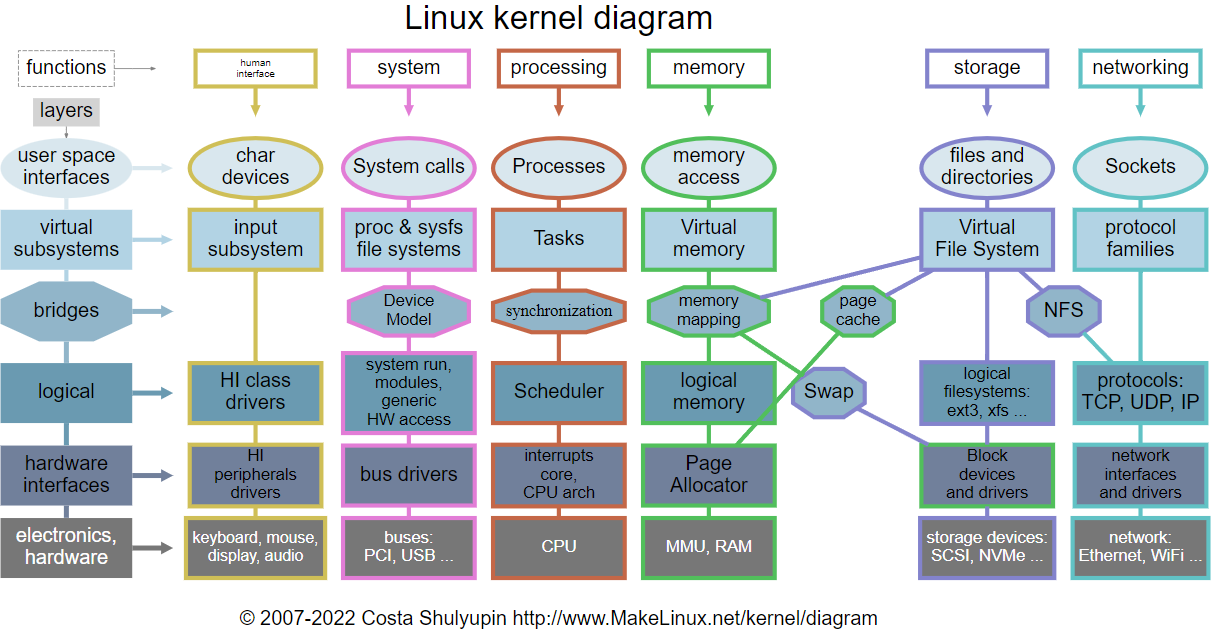
\includegraphics[scale=.45]{images/linux-diagram.png}
    \caption{Diagram representing the modular structure of the Linux Kernel.}
    \label{fig:linux-diagram}
\end{figure}

\noindent However, this flexibility does not provide complete isolation: a loaded module continues to run in kernel space and can access the kernel's internal structures, with the same aforementioned security implications.

Since its first release in 1991, Linux has evolved from a small-scale project into a platform used on a vast number of servers and devices all around the world, as we can see on the following table which sums up the distribution of Linux-powered machines around the world \cite{bib:fosspost}:

\begin{table}[H]
    \centering
    \begin{tabular}{|c|c|}
        \hline
        \textbf{Metric} & \textbf{Linux Share} \\\hline
        Server OS Market (2026 est.) & 51.3\% \\\hline
        Websites (known OS) & 61.3\% \\\hline
        Top 1 Million Web Servers & 96.3\% \\\hline
        Government Data Centers & 64.9\% \\\hline
        Top500 Supercomputers & 100\% \\
        \hline
    \end{tabular}
\end{table}

\noindent This evolution has been accompanied by the introduction of numerous hardware architectures, new drivers and subsystems, which support a broader quantity of features but bring more security and stability issues on the kernel's side. The interfaces exposed to user space are kept as stable as possible, while the kernel's internal APIs may change significantly between different versions.

\subsection{Kernel objects and memory management}

Unlike operating systems such as Windows, where the concept of \textit{kernel object} is formally defined and exposed through a unified object manager \cite{bib:windows-kernel-object}, the Linux kernel does not adopt a single, centralized abstraction for its internal entities but takes advantage of a rich set of well-defined C structures that represent the fundamental components of the system (e.g. processes, files, network sockets, memory regions). Each of these structures encapsulates both the data describing the entity and the state required to manage its lifecycle.

A representative example is \texttt{task\_struct} \cite{bib:sched.h}: this structure is used by the kernel to represent a process or thread. It contains hundreds of fields: scheduling information, memory maps, open file descriptors, credentials, and more; it is one of the most referenced structures throughout the kernel codebase. Similar in spirit are structures such as \texttt{struct socket} \cite{bib:struct-socket} and \texttt{struct sock} \cite{bib:struct-sock} in the networking subsystem, \texttt{struct inode} \cite{bib:struct-inode} for filesystem objects, or \texttt{struct sk\_buff} \cite{bib:struct-sk-buff} for network packets.

These objects are dynamically allocated on the kernel heap through the \textit{slab allocator} \cite{bib:slab-allocator} (in its modern SLUB implementation \cite{bib:slub}), a memory management subsystem optimized for the frequent allocation and deallocation of fixed-size objects. The slab allocator maintains per-type caches of pre-allocated memory, reducing fragmentation and allocation overhead but also, as will be discussed, creating conditions that are relevant to the exploitation of memory corruption vulnerabilities.

Since many of these objects can be referenced simultaneously from multiple kernel subsystems (e.g. a socket can be held by a process, referenced by a pending timer, and pointed to by an active network connection at the same time) their lifetime cannot be tied to a single owner and this is where the reference counting mechanism comes into play. It is efficient, but its correctness relies entirely on every code path that acquires or releases a reference doing so properly. As the kernel grows in complexity and concurrency, maintaining this invariant across all subsystems becomes increasingly difficult and subtle errors in reference counter management can cause the counter to reach zero prematurely, triggering the deallocation of an object that is still reachable from some other part of the kernel.

\subsection{Use-after-free vulnerabilities in the Linux kernel}

Use-after-free vulnerabilities are particularly relevant in the Linux kernel because many kernel objects are dynamically allocated, shared among different subsystems and accessed concurrently by multiple execution contexts (e.g. sockets, network objects, device structures). Their lifetime, as described in section \ref{sec:refcount}, is often managed through mechanisms like reference counting which, in case of wrong manipulation, can produce dangling pointers and subsequent use-after-free exploits.

As stated previously, the consequences of errors like these are generally more severe than in a normal user-space program, since kernel code executes with high privileges. Detecting these vulnerabilities is complicated by the structure of the kernel itself. The allocation, use and release of an object may occur in different context and the relevant sequence of operation is likely not visible within a single control-flow path (this includes the thread concurrency problem seen in section \ref{sec:exploiting-uaf-refcount}). 

These characteristics make automated kernel analysis particularly complex. Detection tools have to deal with code spread across multiple modules that interact in a non-linear manner. Their analysis may also be constrained to a specific kernel version or compiler, or require modifications to the build system and, in some cases, full kernel instrumentation. Moreover, the continuous evolution of internal APIs can quickly lead to compatibility issues if the analyzer is not actively maintained. The kernel documentation distinguishes between numerous categories of tools, such as:
\begin{itemize}
    \item \textit{static analyzers}: code analysis by tracking objects' paths without executing the code. An example is UAFX \cite{bib:uafx}, which we tested and discuss in section \ref{uafx}
    \item \textit{sanitizers}: suspect behaviour detection by instrumentating the code through a compiler
    \item \textit{code coverage tools}: measurement of the quantity of code covered by tests
    \item \textit{fuzzing tools}: generation of random inputs in order to test different execution paths for the analyzed software 
    \item \textit{mechanisms for detecting race conditions}: identification of critical code sections where a race condition may happen
\end{itemize}

\subsubsection{LLVM}
Most of the tools we have considered are based on LLVM \cite{bib:llvm}, a modular infrastructure for building compilers and code analysis tools. Its central component is an intermediate representation (generated by a compiler; one of the most used is Clang \cite{bib:clang}), commonly referred to as LLVM IR, on which modifications can be made that are independent of the source language and, to some extent, of the target architecture. 

The use of LLVM is significant in the field of security because it allows analyses and transformations to be incorporated directly into the compilation process (e.g. by adding checks that will be executed at runtime). This integration enables more in-depth analyses than simply processing the source code textually, albeit at the expense of the performance of the system being analysed; however, a system compiled with LLVM will likely not be made available to the end user but will be used solely for analysis purposes.

\section{Existing tools for detecting UAF vulnerabilities}
For all known bugs, there is a wide range of tools described in the academic literature, used either individually or in combination, that serve (or help) to detect them. UAF issues, however, especially when related to reference counting problems, are particularly challenging.
Due to the unpredictable nature of these bugs, the numerous conditions required to exploit them, and the variety of contexts in which they can occur, identifying them is by no means easy. In addition to the identification process itself, other problems may arise, such as large volumes of false positives that can cause a tool to be inaccurate on its own and require human review to distinguish them from true positives, or the need for extreme computational power to run the tool effectively.

Below are some examples of tools capable of analyzing code and detecting use-after-free vulnerabilities. Since each vulnerability exploits different weaknesses, we have compiled a list of tools with different purposes and modes of operation to provide a broader range of options in this regard.

{
    \renewcommand{\arraystretch}{1.5} % Padding verticale
    \begin{table}[H]
        \small
        \centering
        \begin{tabular}{|c|c|c|c|c|}
            \hline
            \textbf{Tool} & \textbf{\makecell{LLVM//based}} & \textbf{\makecell{Usable in\\kernel}} & \textbf{\makecell{Public\\source}} & \textbf{\makecell{Supports\\refcount}}\\\hline
            \textbf{UAFX} \cite{bib:uafx} & Yes & Yes & Yes & No \\\hline
            \textbf{CountDown} \cite{bib:countdown} & Yes & Yes & Yes & Yes \\\hline
            Infer \cite{bib:infer} & Yes (+ Clang) & Yes & Yes & No \\\hline
            Clang Static Analyzer \cite{bib:clang} & Yes & Yes & Yes & No \\\hline
            Syzkaller \cite{bib:syzkaller} & Yes & Yes & Yes & No \\\hline
            GCC-fanalyzer \cite{bib:gcc} & No & No & Yes & No \\\hline
            CRed \cite{bib:cred} & Yes & No & No & No \\\hline
            Cppcheck \cite{bib:cppcheck} & Yes & No & Yes & No \\\hline
            SVF-derived tools \cite{bib:svf} & Yes & No & Yes & No \\\hline
            FreeWill \cite{bib:freewill} & Yes & No & No & Yes \\\hline
            LinkRID \cite{bib:linkrid} & Yes & Yes & No & Yes \\\hline
            CRCount \cite{bib:crcount} & Yes & No & No & Yes \\\hline
            UAFChecker \cite{bib:uafchecker} & Yes & No & No & No \\\hline
            DCUAF \cite{bib:dcuaf} & Yes & Yes & No & No\\\hline
            SinkFinder \cite{bib:sinkfinder} & Yes & No & No & Yes \\\hline
            Goshawk \cite{bib:goshawk} & Yes & Yes & Yes & No \\\hline
            CID \cite{bib:cid} & Yes & Yes & No & Yes \\\hline
        \end{tabular}
    \end{table}
}

\noindent In the next sections, we will describe the tools that are relevant for this work. There were two tools specifically designed to detect UAF bugs in the Linux kernel: CountDown and CID. Unfortunately, CID does not have publicly available source code, and, as with other tools that do not meet this criterion, we decided to exclude them from the selection.\\
Since our focus was on a use-after-free vulnerability involving a reference-counting issue, we also excluded some tools whose papers clearly stated that they would not be effective for this purpose.\\
Finally, we excluded the tools that would not have worked on the kernel because they were designed for smaller, less complex sections of code.\\
After considering these factors, the decision was made to choose UAFX and CountDown.

\subsection{UAFX}\label{uafx}
UAFX is a static analyzer, presented at NDSS 2025 \cite{bib:uafx}, designed to detect \textit{cross-entry} (non-linear) use-after-free vulnerabilities in the Linux kernel. The term "cross-entry" refers to conditions in which the deallocation and subsequent use of an object occur through different entry points (e.g system calls, callbacks, driver interfaces). In such cases, the link between the deallocation point and the usage point may involve parts distributed across distinct execution paths, making it difficult to detect using analyzers limited to a single function or a single call chain (i.e. where memory allocation, usage, and deallocation occur in a linear pattern). UAFX's approach is based on achieving two main macro-objectives:

\begin{itemize}
    \item \textbf{Escape-Fetch-based Cross-Entry Alias Analysis}
    \item \textbf{Systematic Partial-Order Constraint-based UAF Validation}
\end{itemize}

\noindent We describe them with reference to the following figure:

\begin{figure}[h]
    \centering
    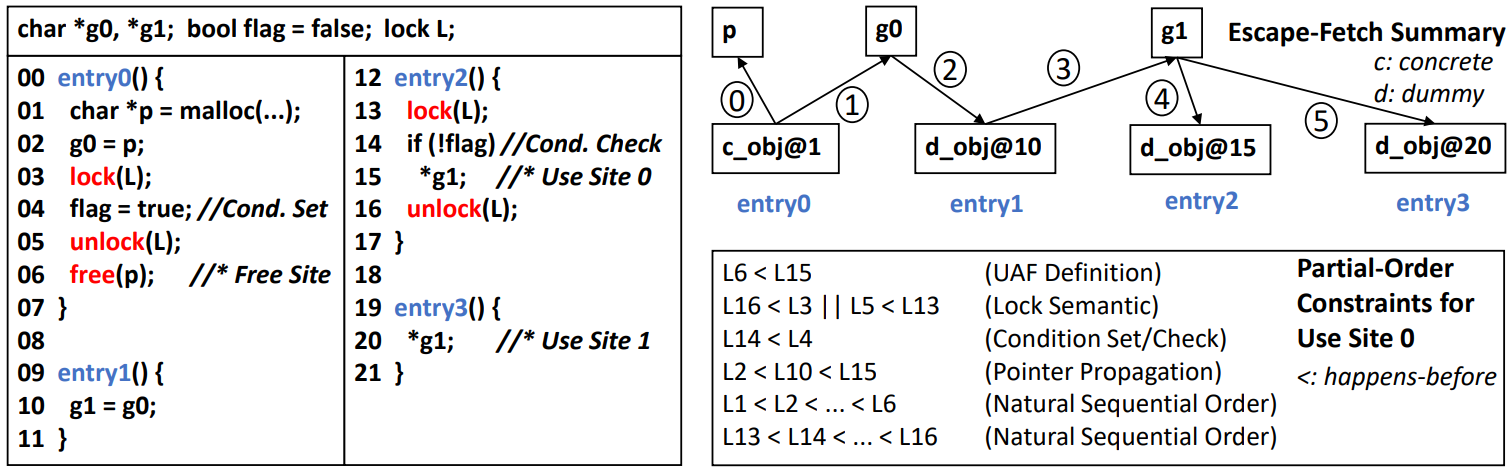
\includegraphics[scale=.4]{images/uafx-example.png}
    \caption{Example of code entry points and how they are handled by UAFX.}
    \label{fig:uafx-example}
\end{figure}

\subsubsection{Escape-Fetch-based Cross-Entry Alias Analysis}
UAFX treats object assignments to pointers as \emph{escapes} and retrievals (from "unknown" areas) as \emph{fetches}. UAFX attempts to construct Escape-Fetch Paths (EFPs) to define aliases that track memory allocation, usage, and deallocation from different access points. This is necessary because, from the perspective of a single function, an object may have an unknown origin (as is commonly the case with an externally initialized pointer, such as \texttt{g1} in \texttt{entry3}).

\subsubsection{Systematic Partial-Order Constraint-based UAF Validation}
Once the aliases/paths have been confirmed, UAFX verifies that the conditions for a UAF actually exist.
If, for example, there is a check on a flag (\texttt{entry0}, \texttt{entry2}) that is manipulated by multiple entry functions and used to prevent a UAF on a critical pointer, that path must be discarded.

\subsubsection{Workflow}
We can break down UAFX's workflow as follows:
\begin{enumerate}
    \item \textbf{Identifying entry functions.} This is done semi-automatically, starting with:
    \begin{itemize}
        \item \textit{General call analysis}: functions that serve as entry points typically have no callers in the program, so they are candidates.
        \item \textit{Software-based heuristics}: the paper uses drivers as an example; these typically have entry points in a \texttt{file\_operations} structure, which makes them easy to identify.
    \end{itemize}
    After these initial automated steps, a manual review is conducted to exclude unnecessary candidates or to add others.

    \item \textbf{Code analysis and summary for each entry.} The entry functions are analyzed, and all escape/fetch objects, critical regions, and condition sets/checks (such as the flag in the example) are identified. UAFX generates a summary of all possible paths (in Figure \ref{fig:uafx-example}, the graph in the upper right).

    \item \textbf{Cross-entry detection of free and use sites with aliases.} UAFX considers all sites where memory regions are freed and used as potential candidates for UAF. In the example, with the path \texttt{entry0}-\texttt{entry3}, defined as follows (between the \textit{free} operation on line 6 and the \textit{use} operation on line 20):
    \begin{center}
        (c\_obj@1 $\longrightarrow$ g0 $\longrightarrow$ d\_obj@10 $\longrightarrow$ g1 $\longrightarrow$ d\_obj@20)
    \end{center}
    there is a potential UAF.

    \item \textbf{UAF Validation.} UAFX considers all candidates and evaluates their constraints within the path (order, locks, set/check conditions) to determine whether each one is actually a vulnerability.
    It also verifies that the free and use sites actually access the same object, taking into account the entire escape-fetch path.
    For this purpose, SMT solvers can be used (the paper cites z3 \cite{bib:z3} as an example).
\end{enumerate}

\subsubsection{Thread tracking}
Since some UAFs are caused by race conditions, UAFX recognizes two types of thread-related lifecycles:
\begin{itemize}
    \item \textbf{Thread creation}: calls that create child threads (\texttt{pthread\_create}, \texttt{fork}). UAFX retrieves information from these events (e.g., the thread's entry function or parameters)

    \item \textbf{Thread joins} (\texttt{pthread\_join}, \texttt{wait}): events that ensure threads exit before a certain point in the parent thread. UAFX pairs each exit event with its corresponding creation event to track the entire thread lifecycle.
\end{itemize}

\subsubsection{UAFX limitations and extensions}

Although UAFX is designed to automatically identify use-after-free vulnerabilities, its analysis deliberately excludes some classes of candidates in order to preserve high precision and limit the number of false positives.

A first limitation concerns the identification of entry functions. As described previously, UAFX automatically considers functions with no callers as potential entry points, but relevant functions may themselves be invoked by other functions and therefore not satisfy this criterion. UAFX addresses this limitation by allowing additional entry functions to be manually included in the candidate set during the second stage of the identification process.

A more significant limitation concerns reference-counting mechanisms. As explicitly discussed by the authors in the \textit{Reference Count Mechanisms} section of the UAFX paper \cite{bib:uafx}, candidates involving reference counting are intentionally excluded from the analysis. Tracking the lifetime of reference-counted objects introduces additional complexity and may produce a large number of false positives. The authors therefore favor higher precision at the cost of reduced recall for this class of lifetime-management errors.

This limitation does not imply that reference-count-related vulnerabilities cannot be addressed through static analysis. Other tools focus specifically on the analysis of reference-counting mechanisms and may complement the approach adopted by UAFX. In particular, LinKRID \cite{bib:linkrid}, CRCount \cite{bib:crcount}, and FreeWill \cite{bib:freewill} are discussed in relation to the identification of reference-counting errors. Their analyses could potentially be combined with or used to extend UAFX, although doing so would require adapting the respective analyses and reconciling their different representations of object lifetime and reference-management operations.

Such an extension would broaden the class of lifetime errors considered by UAFX, potentially improving its ability to detect use-after-free conditions originating from incorrect reference-count management. However, this would also introduce the precision-recall trade-off that UAFX deliberately avoids in its original design.

\subsection{CountDown}
CountDown is a fuzzer for the Linux kernel, presented at CCS 2024 \cite{bib:countdown} and, unlike UAFX, it's specifically designed to detect memory timing errors caused by incorrect handling of reference counters. Unlike traditional fuzzers, which are primarily driven by code coverage, CountDown uses operations on reference counters as feedback to identify sequences of system calls that could potentially alter the lifecycle of those same objects. The tool is built on top of Syzkaller \cite{bib:syzkaller} (an open source, unsupervised, coverage-guided kernel fuzzer developed by Google) and extends its strategies for generating and mutating test programs.

During execution, CountDown instruments the kernel to associate increments, decrements, and accesses to reference counters with the system calls that triggered them. Based on this information, it establishes relationships between system calls that operate on the same counters and assigns them a higher probability of being combined in the generated tests. The tool can also repeatedly insert operations that decrement a counter, in an attempt to trigger the object's deallocation, followed by operations that continue to access it. In this way, fuzzing is directed toward sequences that can more effectively expose UAFs caused by incorrect operations on counters.

CountDown's approach is based on the idea of refcount-driven fuzzing to achieve two macro-objectives:
\begin{itemize}
    \item \textit{Identification of refcount-based relationships between syscalls}: instead of relying solely on syscall signatures or coverage, CountDown correlates syscalls that operate on the same object (\textit{shared refcounts}).

    \item \textit{Systematic exposure of UAF bugs}: through targeted mutations, the tool attempts to force an object's refcount to zero and subsequently access that object via syscalls that share its reference.
\end{itemize}

\subsubsection{Workflow}
CountDown's workflow can be broken down into three main phases:
\begin{enumerate}
    \item \textbf{Kernel instrumentation and logging}: CountDown instruments the refcount APIs in the Linux kernel to log every refcount operation using a 4-element tuple:
    \begin{center}
        $<S, O, \delta, V>$
    \end{center}
    where a syscall S updates the refcount O by a value $\delta$. V is the final value.

    The instrumented APIs are listed in the following table:

    \begin{center}
        \begin{tabular}{|c|c|}
            \hline
            \textbf{Name} & \textbf{Description} \\\hline
            \texttt{refcount\_set} & set refcount to the given value \\\hline
            \texttt{refcount\_add} & add the given value to refcount \\\hline
            \texttt{refcount\_inc} & increase refcount by 1 \\\hline
            \texttt{refcount\_dec} & decrease refcount by 1 \\\hline
            \texttt{refcount\_add\_not\_zero} & add given value to refcount if refcount is not 0 \\\hline
            \texttt{refcount\_inc\_not\_zero} & increment if the refcount is not 0 \\\hline
            \texttt{refcount\_dec\_not\_one} & decrement if the refcount is not 1 \\\hline
            \texttt{refcount\_dec\_if\_one} & decrement if the refcount is 1 \\\hline
            \texttt{refcount\_dec\_and\_test} & decrement refcount and check if result is 0 \\\hline
            \texttt{refcount\_sub\_and\_test} & subtract value from refcount and check it with 0 \\\hline
        \end{tabular}
        \label{table:refcounts}
    \end{center}
    
    To identify the same object across different virtual machines (VMs), it uses a checksum of the call stack at the time of the object's initialization through \texttt{refcount\_set}.

    CountDown creates a RAI map (\texttt{refcount-address-ID}) to link the addresses of the refcounts with their refcount IDs.\\
    When a refcount is initialized, a new entry in the RAI map is created with its address and ID.\\
    When a refcount reaches zero, the entry is removed from the map.\\
    When a refcount is incremented or decremented, CountDown searches the address in the map to find its ID and records the operation.

    During fuzzing, to connect refcount operations with syscalls, CountDown needs to record the Syzkaller syscall number (NR) for each operation. This is done in a thread-safe manner in order to avoid race condition, since the Linux kernel utilizes multiple threads to execute parallelized syscalls.

    While tracking the refcount values, CountDown considers that one syscall may modify a refcount many times, but it only cares about the final variation ($\delta$). In order to do so, every refcount API listed in table \ref{table:refcounts} is modified to record every single refcount change.
    This data is kept in a two-dimension table (one for the syscall number, one for the refcount ID), in which every entry records the current $\delta$ and the current $V$. 

    \item \textbf{Reworking relationships between system calls}: CountDown constructs multiple relations among syscalls and refcounts starting from the refcount operations mapped in the 4-tuple format $(S, O, \delta, V)$.
    
    First, it identifies syscalls that effectively change the refcount of any object. It remaps a set of 4-tuples in a new map, where the key is the refcount ID and the value is a set of syscalls and their changes to the refcount ($\delta$), avoiding relations between syscalls from different programs (which can quickly become unrealiable).
    
    Based on the shared refcounts, every relation is reworked in a new one defined as \texttt{RefcntRelation}. The assumption is that, if two syscalls access the same refcount within one execution, they have a stronger relation with respect to triggering more complicated refcount operations. Each syscall set associated with a specific refcount is then split into a set of syscalls pairs. Following that, CountDown creates the syscall relation table, where each unique pair of syscalls has an entry and the value is the number of shared refcounts accessed by both.
    
    \begin{center}
        \begin{figure}[h]
            \centering
            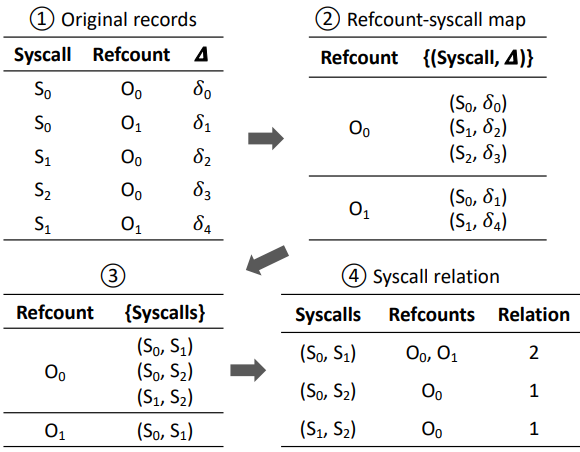
\includegraphics[width=0.7\linewidth]{images/countdown-step2.png}
            \caption{Example of refcount-based syscall relation construction.}
            \label{fig:countdown-step2}
        \end{figure}
    \end{center}
    
    As explained in the paper, this newly constructed relation is more efficient in detecting refcount-related UAF bugs. However, the kernel code base is very large and refcount operations are not densely distributed. To solve the problem, the \texttt{RefCntRelation} is merged with the Syzkaller's standard \texttt{SyzRelation} and handled based on the fuzzing time. At the beginning of fuzzing, CountDown assigns a high priority to the original coverage-based relation to quickly explore more kernel code. As time goes on, it allocates more weight to CountDown's own relation so that the fuzzer can focus on testing complex refcount operations. This can be represented as the following formula:

    \begin{center}
        $OverallRelation = log_2(SyzRelation) + k * log_2 (RefcntRelation)$
    \end{center}

    $k$ starts with a small value and is incremented every time after testing a fixed number of test cases.

    Since fuzzers are non-deterministic, different kernel instances can gather different relations. When a new one is received from one VM, CountDown synchronizes it across all instances (to ensure that the other instances can directly make use of it) by fetching each VM's report, merging them and then distributing the result to all instances.

    \item \textbf{Guided program mutation}: CountDown uses the learned relationships to generate new programs. It starts by using the mutators from previous fuzzing tools (like Syzkaller) to mutate the program. Having assigned higher weights to refcount-based relations, the mutation will prefer combining syscalls that are strongly related regarding refcount operations.  

    Then it creates a new mutator that combines refcount-related syscalls more aggressively. CountDown chooses one target program and runs it in order to collect all accessed refcounts. It will update the refcount-syscall map if the execution triggers new records. To mutate the program, it will randomly select a refcount from the collected set. If a refcount was accessed multiple times, it will have a higher probability to be selected. 

    CountDown then searches the map for syscalls that operate on this refcount and selects one for insertion into the program, which is done reusing Syzkaller's logic, preferring a later position, because the syscalls at the beginning may work on the initialization of resources and refcounts.

    In addition to new code coverage, CountDown considers any program that exhibits a new \texttt{(syscall, refcount)} pair never seen before to be "interesting" and saves it for future changes. This is done while fuzzing through checking whether the execution triggers new code coverage or a new refcount operation, which was previously missed. If that's the case, it saves the new program into the input queue for further mutations and updates the refcount-syscall map with the new entry.

    As a final but important point, a triggered refcount error will not immediately result in a memory error. CountDown needs to trigger more operations to make the kernel release the object and access it through dangling references. It does so by inserting more refcount-related syscalls into the executed program in order to reduce the gap between a refcount bug and a UAF, so that sanitizers like KASAN can capture it.
\end{enumerate}

\subsubsection{Limitations}
Although CountDown is optimized to detect UAFs with refcounts, it still has some limitations:
\begin{itemize}
    \item \textbf{Generic refcounts}: some refcounts (such as those in the AppArmor security module) are used by nearly all syscalls, creating "noise" and artificial relationships that CountDown must filter out to maintain accuracy.

    \item \textbf{Coverage trade-off}: because it focuses heavily on refcount logic, CountDown may record slightly lower total code coverage (approximately 1.8\% – 4.3\% less) than Syzkaller, as it ignores paths unrelated to object management.

    \item \textbf{Instrumentation overhead}: although optimized through selective logging (excluding interrupts and asynchronous tasks), the constant monitoring of every refcount operation introduces a higher computational load than traditional fuzzing.
\end{itemize}